\section{Описание задачи и методологии работы}
\subsection{Задача и набор данных}
Выбранная для тестирования методов задача заключается в определении, является ли элемент видеопотока телевизионной рекламой. Наша группа не занималась получением признакового описания из видеороликов, а лишь проводила эксперименты на готовом наборе данных, полученном исследователями в \cite{vyas}. Авторы указанной работы преобразовали 150 часов видео с 5 новостных каналов (BBC, CNN, CNN-IBN, NDTV, TIMES NOW) в признаковые описания коротких видеофрагментов, упорядоченных хронологически. Набор данных включает визуальные (длительность фрагмента, распределение разности кадров, распределение движения, распределение текста на экране и процент движущихся границ объектов на видео) и аудиопризнаки (спектральные характеристики аудиосигнала и bag of audio words). Каждому объекту в наборе данных присвоена метка класса: \(+1\) --- фрагмент является рекламой, \(-1\) --- не является. В таблице~\ref{table:class-distr} указаны соотношения классов в данных каждого из каналов:

\begin{table}
    \centering
    \begin{tabular}{|p{4cm}||c|c|c|c|c|}
    \hline
    Канал & BBC & CNN & CNN-IBN & TIMES NOW & NDTV \\ \hline
    Число объектов & 17720 & 22545 & 33117 & 39252 & 17051 \\ \hline
    \% объектов, соответствующих рекламе & 47.5 & 63.9 & 65.5 & 64 & 73.7\\
    \hline
    \end{tabular}
    \caption{Соотношение классов в наборе данных}
    \label{table:class-distr}
\end{table}

\subsection{Методология}
При рассмотрении методов отбора признаков и эталонов нас интересовало то, как их работа отражается на качестве классификации базовых методов машинного обучения и на времени, требующемся для их обучения. Исходя из этого, мы структурировали эксперименты следующим образом:
\begin{enumerate}
    \item Использование базовых методов машинного обучения\\
    Были проведены эксперименты с 5 базовыми методами (см.~\ref{sec:base-methods}) на данных с каждого видеоканала, с изменением одного параметра по некоторой сетке. Для каждого сочетания (метод, канал, значение параметра) была проведена 10-кратная кросс-валидация, в результате которой были получены среднее значение и стандартное отклонение для качества классификации и времени обучения. На основе результатов данной работы мы выбрали по одному значению параметров для каждого метода (из тех, которые имеют параметры) и использовали их в следующих частях работы.
    \item Использование методов отбора признаков\\\label{item:feature-selection}
    Были проведены эксперименты с некоторыми методами отбора признаков по схеме, аналогичной предыдущему пункту, с тем отличием, что в данном случае варьировался параметр метода отбора признаков.
    \item Использование методов отбора эталонов\\
    Аналогично п.\ref{item:feature-selection}.
\end{enumerate}

\subsection{Используемые методы}\label{sec:base-methods}
Мы выбрали 5 методов машинного обучения в качестве базовых, в этом разделе приводятся их описания и результаты, показанные методами для разных параметров.

\subsubsection{\(k\) ближайших соседей}
\(k\)NN --- простой метрический метод, относящий \(\mathbf{x}\) в мажоритарный класс \(k\) ближайших (в нашем случае в евклидовой метрике) соседей из обучающей выборки. Он относится к категории методов так называемого ленивого обучения --- фаза обучения у него состоит лишь в сохранении тестовой выборки полностью. При классификации он проходит по всем объектам обучающей выборки, вычисляя расстояния до классифицируемого объекта, что может выливаться в длительное время работы. Использованная нами реализация метода сохраняет обучающую выборку в KD-дерево, что несколько нивелирует данный негативный эффект. Известно, что \(k\)NN может показывать неудовлетворительные результаты в задачах с сильно многомерным пространством признаков, из-за того, что ближайшие к классифицируемому векторы все оказываются на примерно одинаковом расстоянии от него в евклидовой метрике \cite{beyer}. Также, ленивость \(k\)NN выливается в высокие требования к объёму памяти при работе с большими наборами данных. Эти особенности обуславливают наш интерес к методу \(k\)NN в рамках данной работы.

В тестовых запусках использовались значения параметра \(k\in\{1,3,5,\dotsc,101\}\). На рис.~\ref{fig:knn-base} представлены зависимости качества классификации и времени обучения от \(k\) для разных каналов.
\begin{figure}[h!]
    \centering
	\begin{subfigure}{0.45\textwidth}
		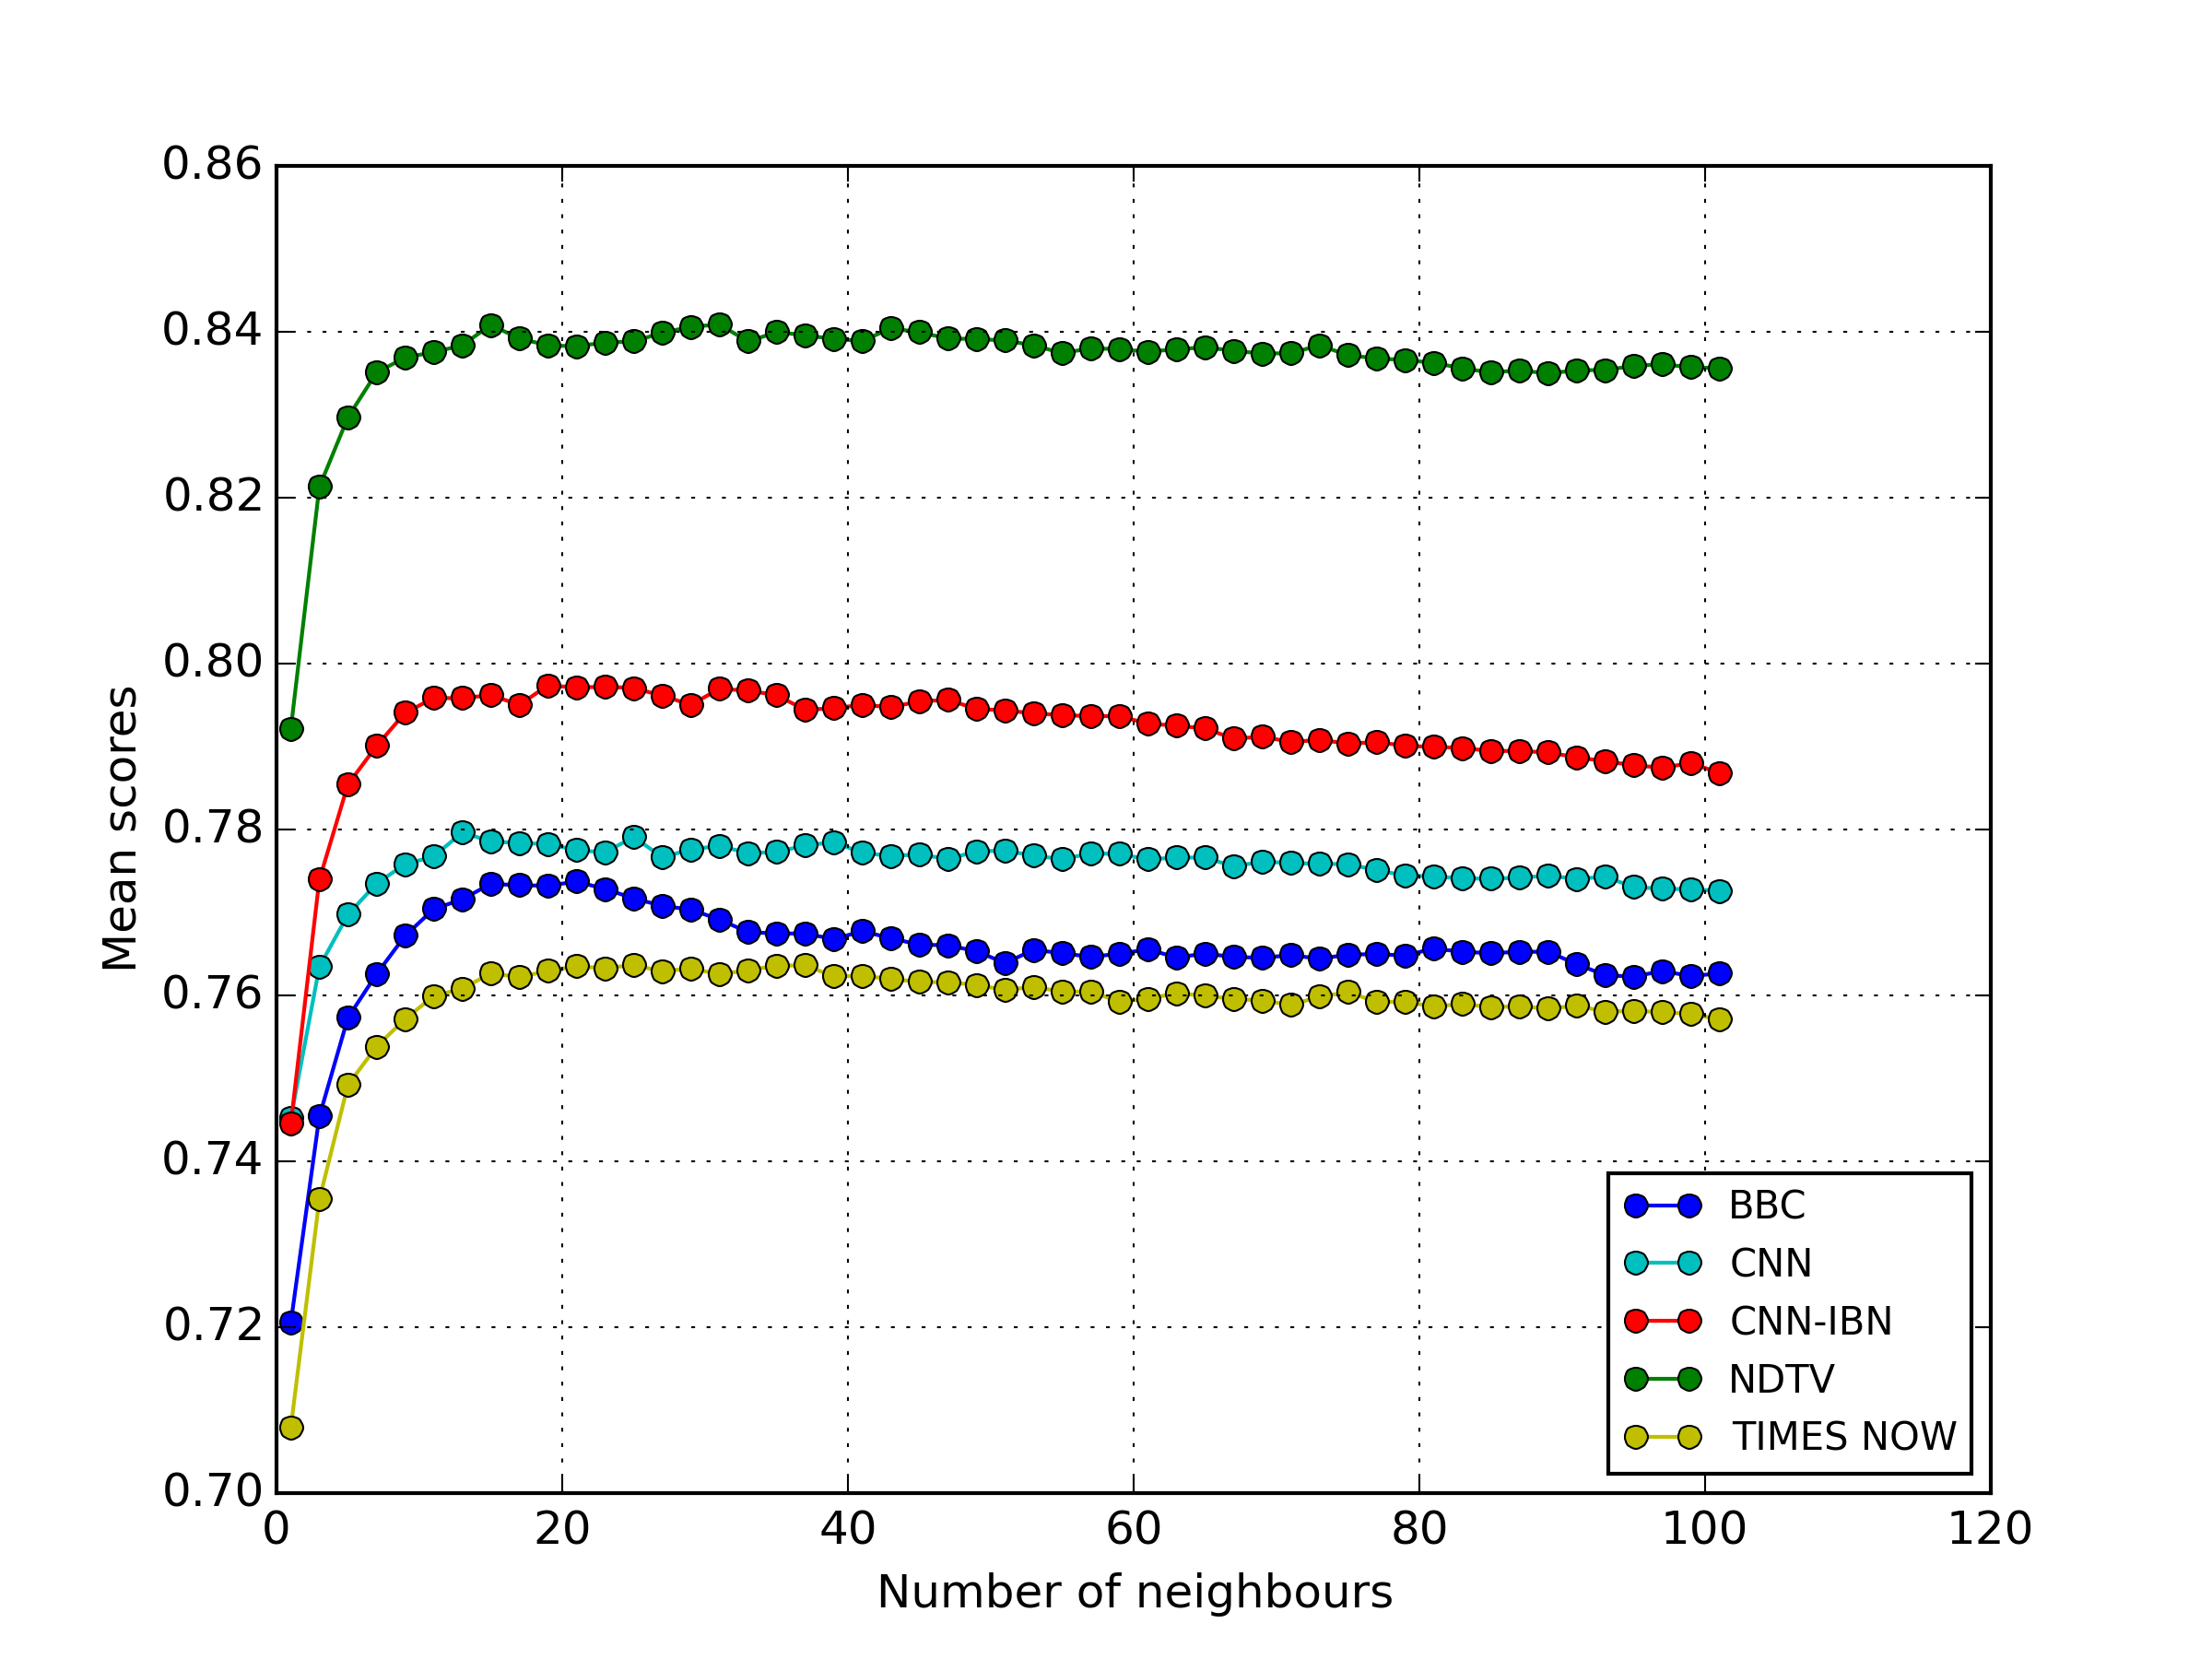
\includegraphics[width=\textwidth]{images/knn.png}
		\caption{Зависимости качества классификации от \(k\) для разных каналов.}
	\end{subfigure}
	\begin{subfigure}{0.45\textwidth}
		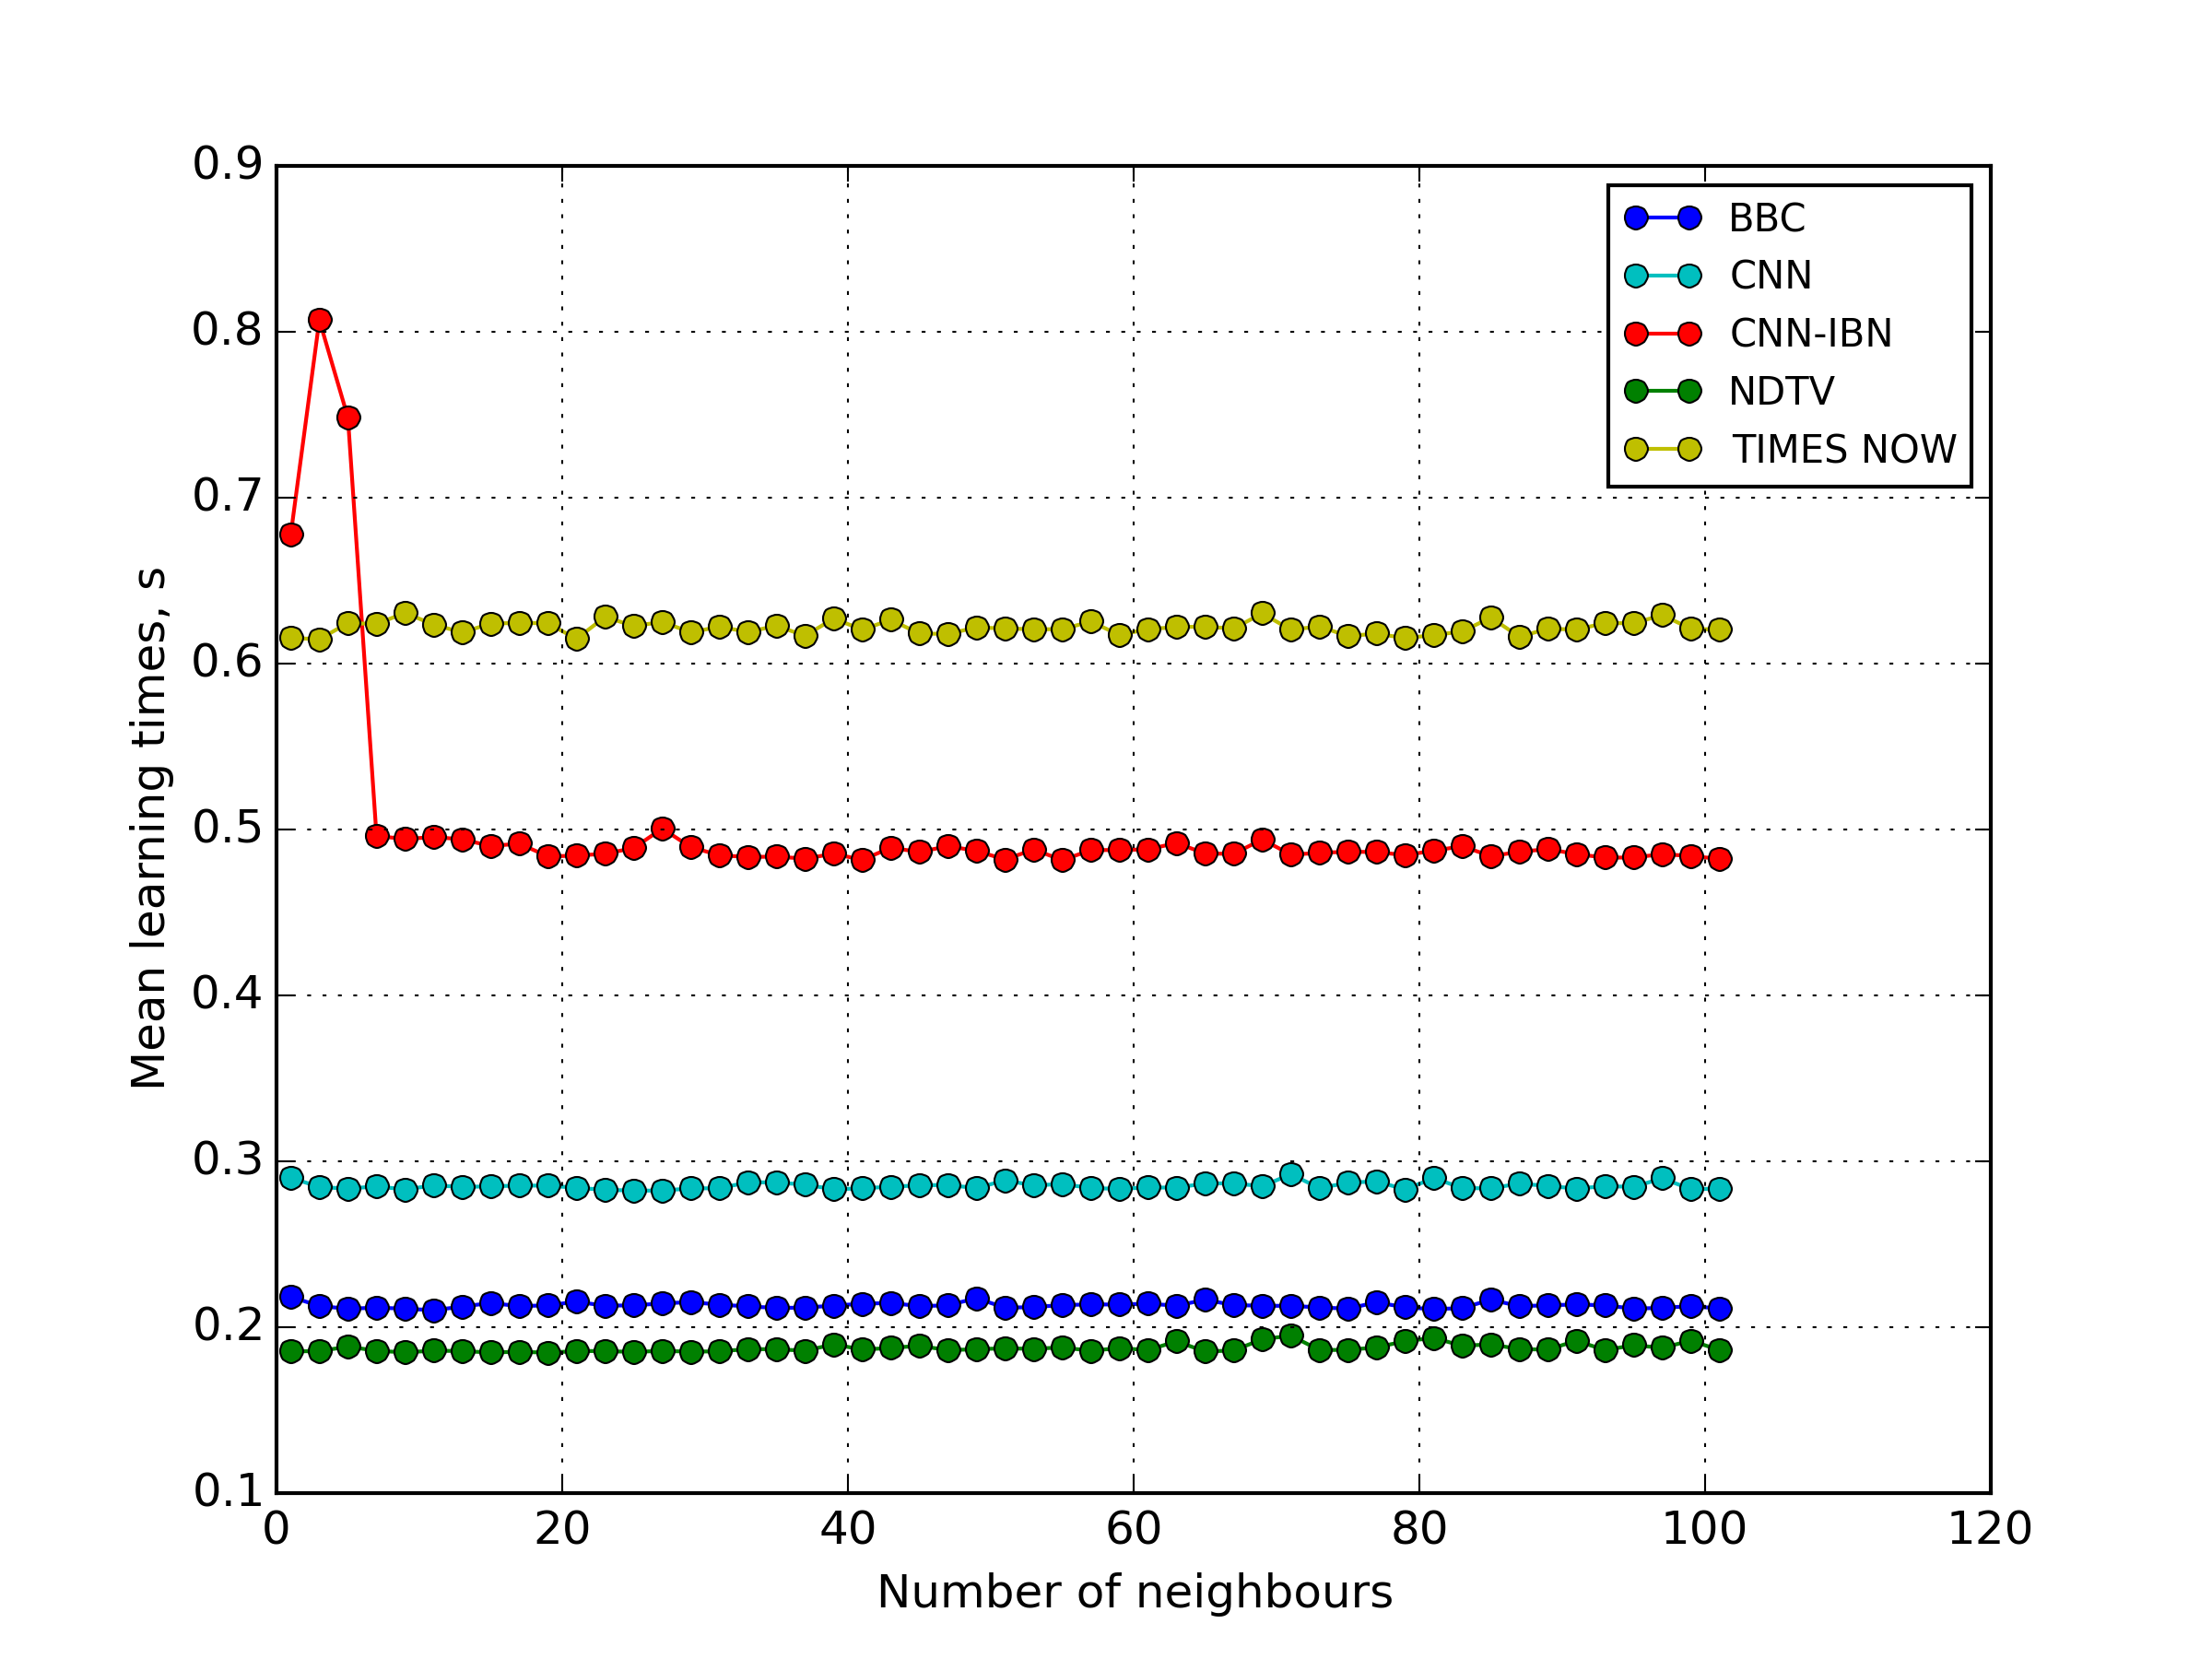
\includegraphics[width=\textwidth]{images/knnTime.png}
		\caption{Зависимости времён обучения от \(k\) для разных каналов.}
	\end{subfigure}
	\caption{Результаты для метода \(k\)NN}\label{fig:knn-base}
\end{figure}

\tbd{Что мы видим на графиках?}

\subsubsection{Линейный дискриминантный анализ}
Линейный дискриминантный анализ в задаче бинарной классификации использует предположения о том, что объекты обоих классов распределены в пространстве признаков нормально, и что матрицы матрицы ковариации этих распределений совпадают. При данных предположениях уравнение разделяющей поверхности, получаемое из принципа максимума апостериорной вероятности, оказывается линейным. Таким образом, в задаче бинарной классификации LDA строит разделяющую гиперплоскость.

LDA в отличие от остальных рассматриваемых методов не имеет настраиваемых параметров. Результаты его работы представлены в сводной таблице~\ref{table:base-all}.

\subsubsection{Машина опорных векторов}
Данный метод является линейным классификатором, он строит гиперплоскость в пространстве признаков, имеющую максимальные зазоры до объектов каждого из классов. Пусть обучающая выборка имеет вид \(\left(X, Y\right)=\{\left(\mathbf{x}_i,y_i\right):i\in\{1,\dotsc,n\}\}\), классы линейно сепарабельны, и разделяющая гиперплоскость описывается \(\mathbf{w}^T\mathbf{x}-b=0\). Зазор ограничивается гиперплоскостями, параллельными искомой: \(\mathbf{w}^T\mathbf{x}-b=\pm1\). Максимизация зазора означает минимизацию \(\|\mathbf{w}\|\) при ограничениях \(y_i\left(\mathbf{w}^T\mathbf{x}_i-b\right)\geqslant1,\;i\in\{1,\dotsc,n\}\). Применением теоремы Куна -- Таккера данная задача сводится к задаче поиска седловой точки функции Лагранжа. При решении этой задачи получаются значения множителей Лагранжа \(\alpha_i, i\in\{1,\dotsc,n\}\), с помощью которых можно вычислить \(\mathbf{w}=\sum_{i=1}^n \alpha_i y_i\mathbf{x}_i\) и \(b=\mathbf{w}^T\mathbf{x}_j-y_j\), где \(j\) --- индекс одного из ненулевых множителей Лагранжа. Лишь несколько \(\alpha_i\) имеют положительное значение, и \(\mathbf{x}_i\), соответствующие таким \(\alpha_i\), называются \emph{опорными векторами}.

В общем случае гарантировать линейную сепарабельность объектов разных классов нельзя, и применяется алгоритм SVM с мягким зазором (soft-margin SVM) \cite{cortes-vapnik}. Отличие от случая линейной сепарабельности заключается во введении \(n\) дополнительных переменных \(\xi_i\), характеризующих ошибки классификации на соответствующих объектах. При этом ограничения принимают вид \(y_i\left(\mathbf{w}^T\mathbf{x}_i - b\right)\geqslant 1-\xi_i,\;i\in\{1,\dotsc,n\}\), а к целевой функции добавляется штраф \(C\sum_{i=1}^n\xi_i\), где \(C\) --- параметр мягкого зазора.

Зачастую параметр мягкого зазора \(C\) подбирается по логарифмической сетке, что мы и проделали. На рис.~\ref{fig:svm-base} представлены результаты данного эксперимента. Из них видно, что среди опробованных значений \(C\) на 4 каналах из 5 наилучший результат SVM показал при \(C=4\), именно это значение было выбрано для дальнейших экспериментов с отбором признаков и эталонов.

\begin{figure}[h!]
    \centering
	\begin{subfigure}{0.45\textwidth}
		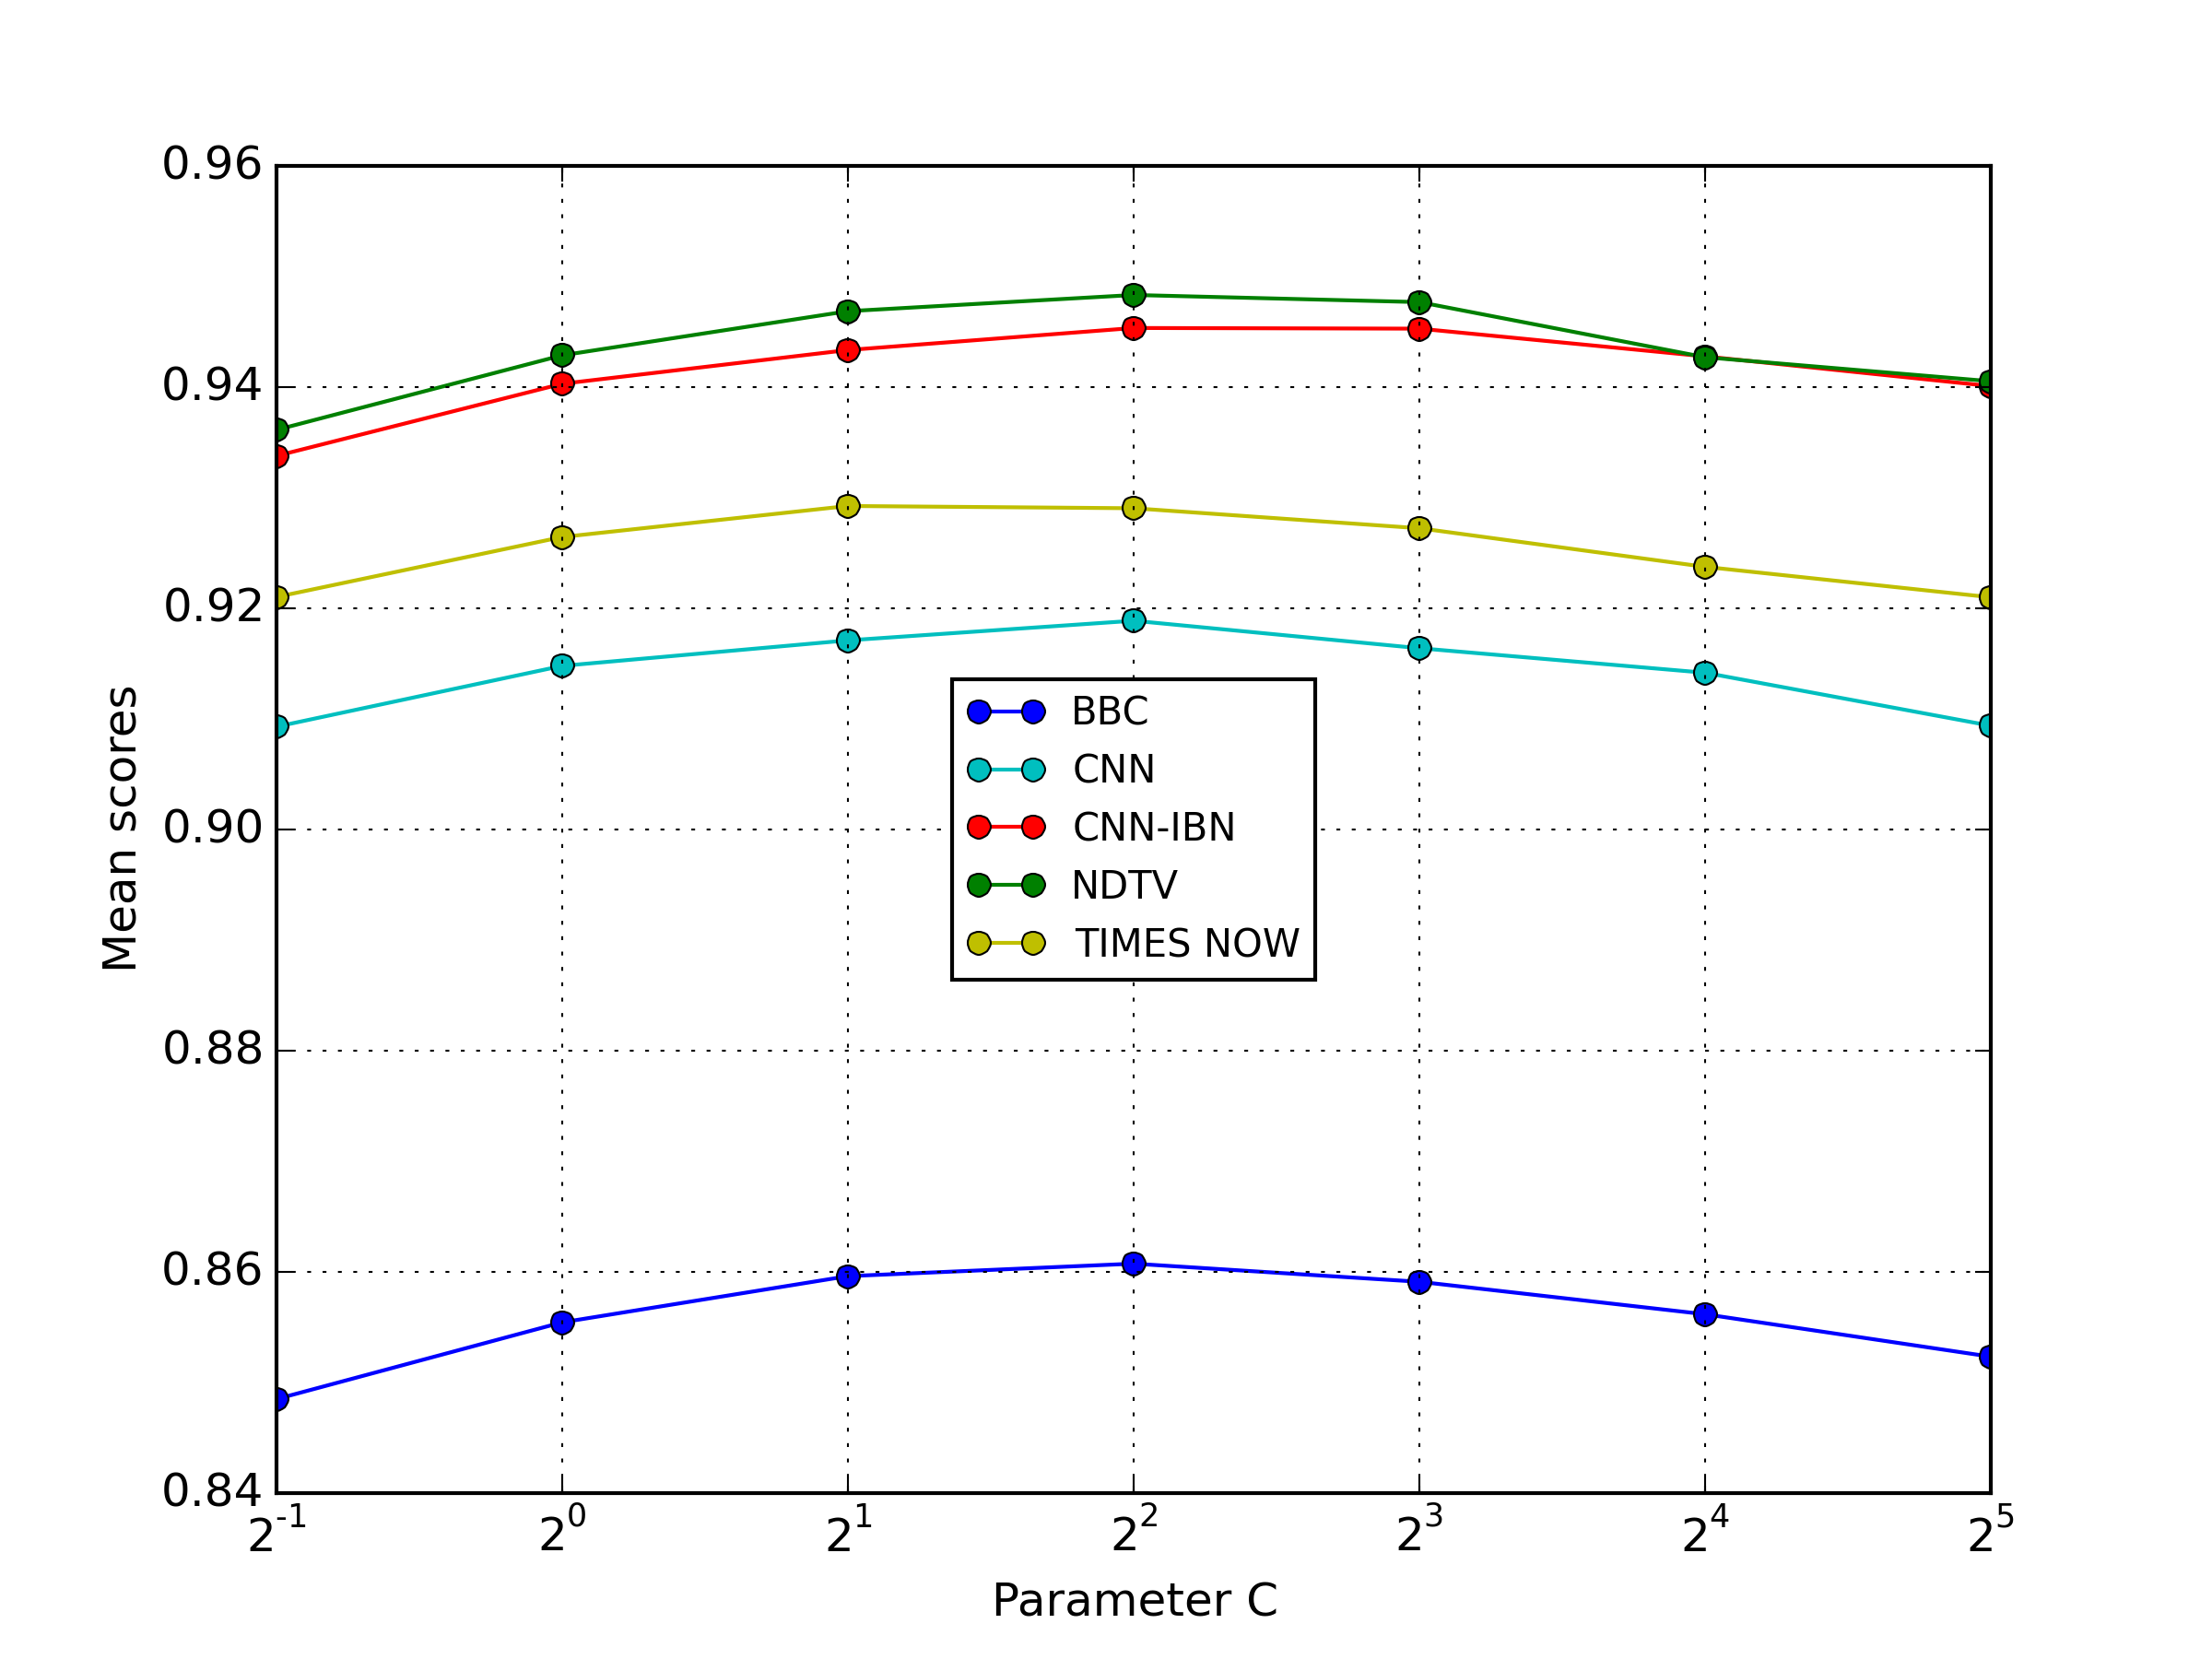
\includegraphics[width=\textwidth]{images/svm.png}
		\caption{Зависимости качества классификации от \(C\) для разных каналов.}
	\end{subfigure}
	\begin{subfigure}{0.45\textwidth}
		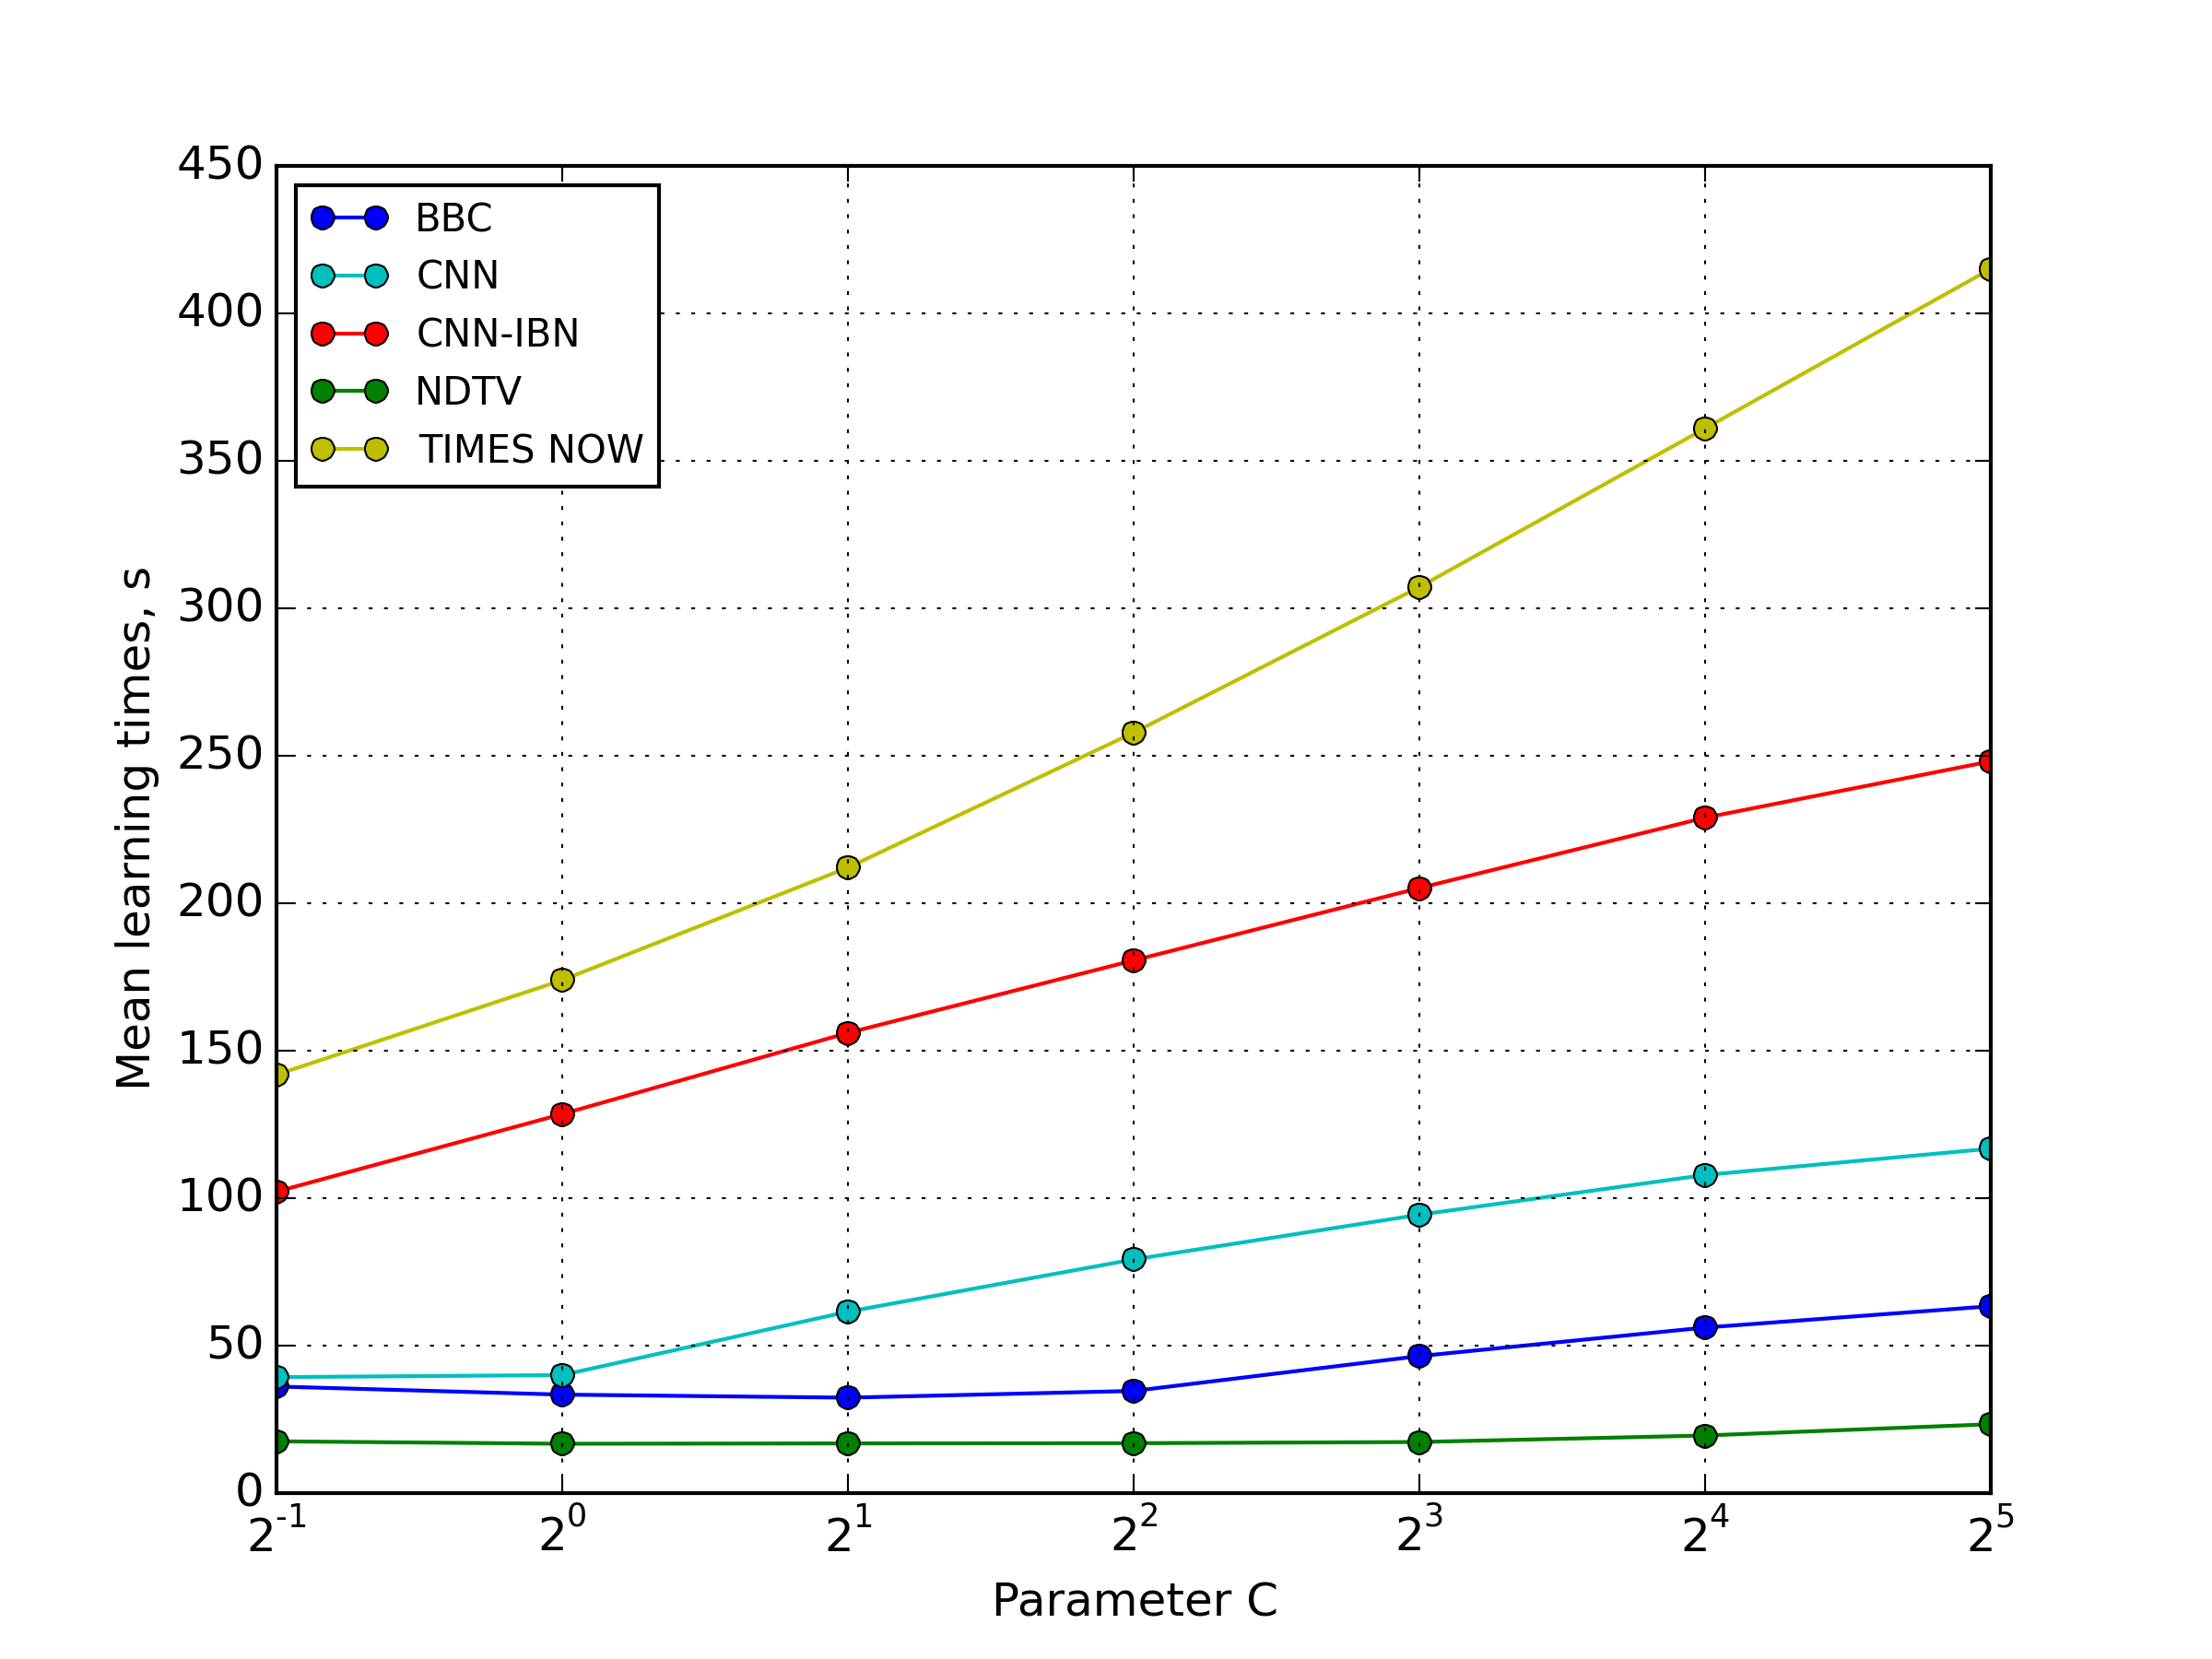
\includegraphics[width=\textwidth]{images/svmTime.png}
		\caption{Зависимости времён обучения от \(C\) для разных каналов.}
	\end{subfigure}
	\caption{Результаты для метода SVM}\label{fig:svm-base}
\end{figure}

\tbd{Что мы видим на графиках?}

\subsubsection{Случайный лес}
Данный алгоритм и является расширением бэггинга для деревьев решений. При использовании бэггинга \(B\) деревьев решений тренируются каждый на своём подмножестве обучающей выборки \(\left(X_b, Y_b\right),\;b=1,\dotsc,B\), полученном из исходной обучающей выборки случайным выбором с повторениями. Ответом классификатора будет класс, за который проголосовало больше всего деревьев. Такое построение классификатора позволяет получить некоррелированные деревья, благодаря чему голосование решает проблемы одиночных деревьев решений с переобучением, вызванные их высокой чувствительностью к выбросам в обучающей выборке. Случайный лес развивает идею бэггинга на шаг дальше. В этом методе модифицируется алгоритм построения дерева: при поиске правила для каждой новой вершины используется случайное подмножество признаков. Если существует сильная зависимости между некоторым признаком и классом объекта, то достаточно большое количество деревьев могут выбрать этот признак при присвоении решающего правила вершине дерева. Таким образом, случайный выбор подмножества признаков позволяет ещё сильнее сократить чувствительность деревьев к шумам.

Были проведены тестовые запуски данного метода для значений \(B\in\{5,10,\dotsc,155\}\). На рис.~\ref{fig:randfor-base} изображены зависимости качества классификации и времени обучения от числа деревьев.
\begin{figure}[h!]
    \centering
	\begin{subfigure}{0.45\textwidth}
		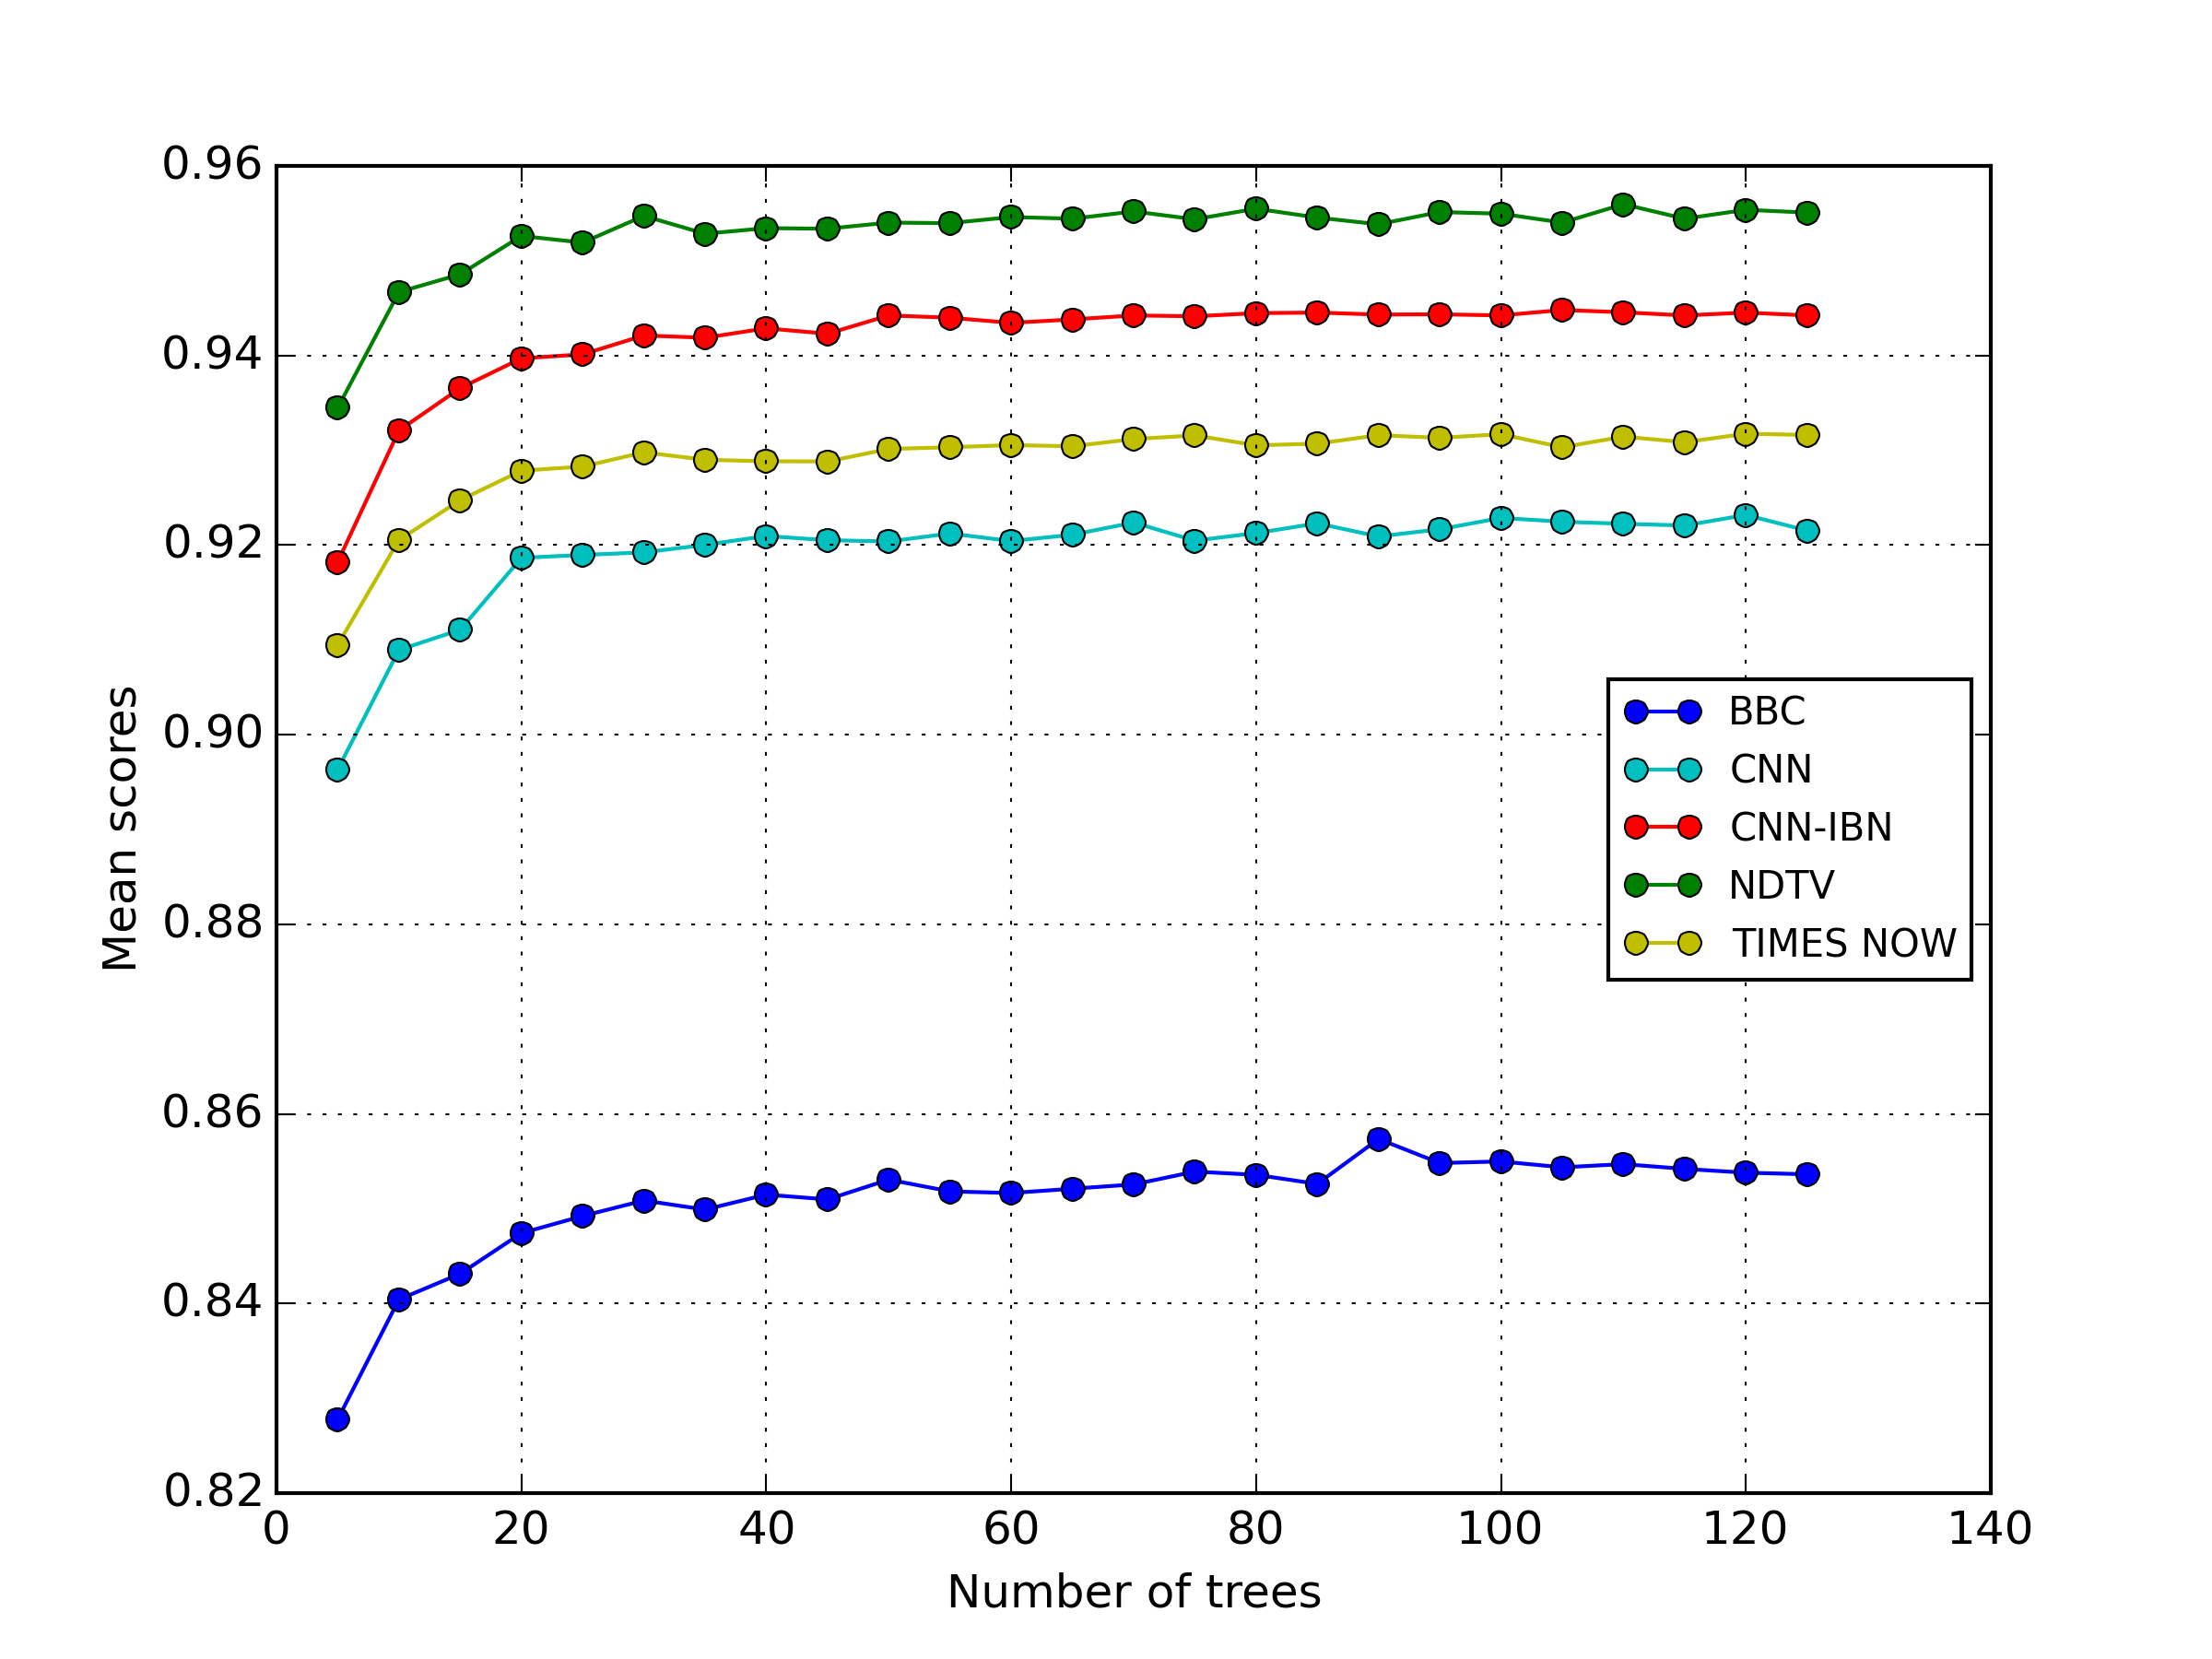
\includegraphics[width=\textwidth]{images/randfor.png}
		\caption{Зависимости качества классификации от числа деревьев для разных каналов.}
	\end{subfigure}
	\begin{subfigure}{0.45\textwidth}
		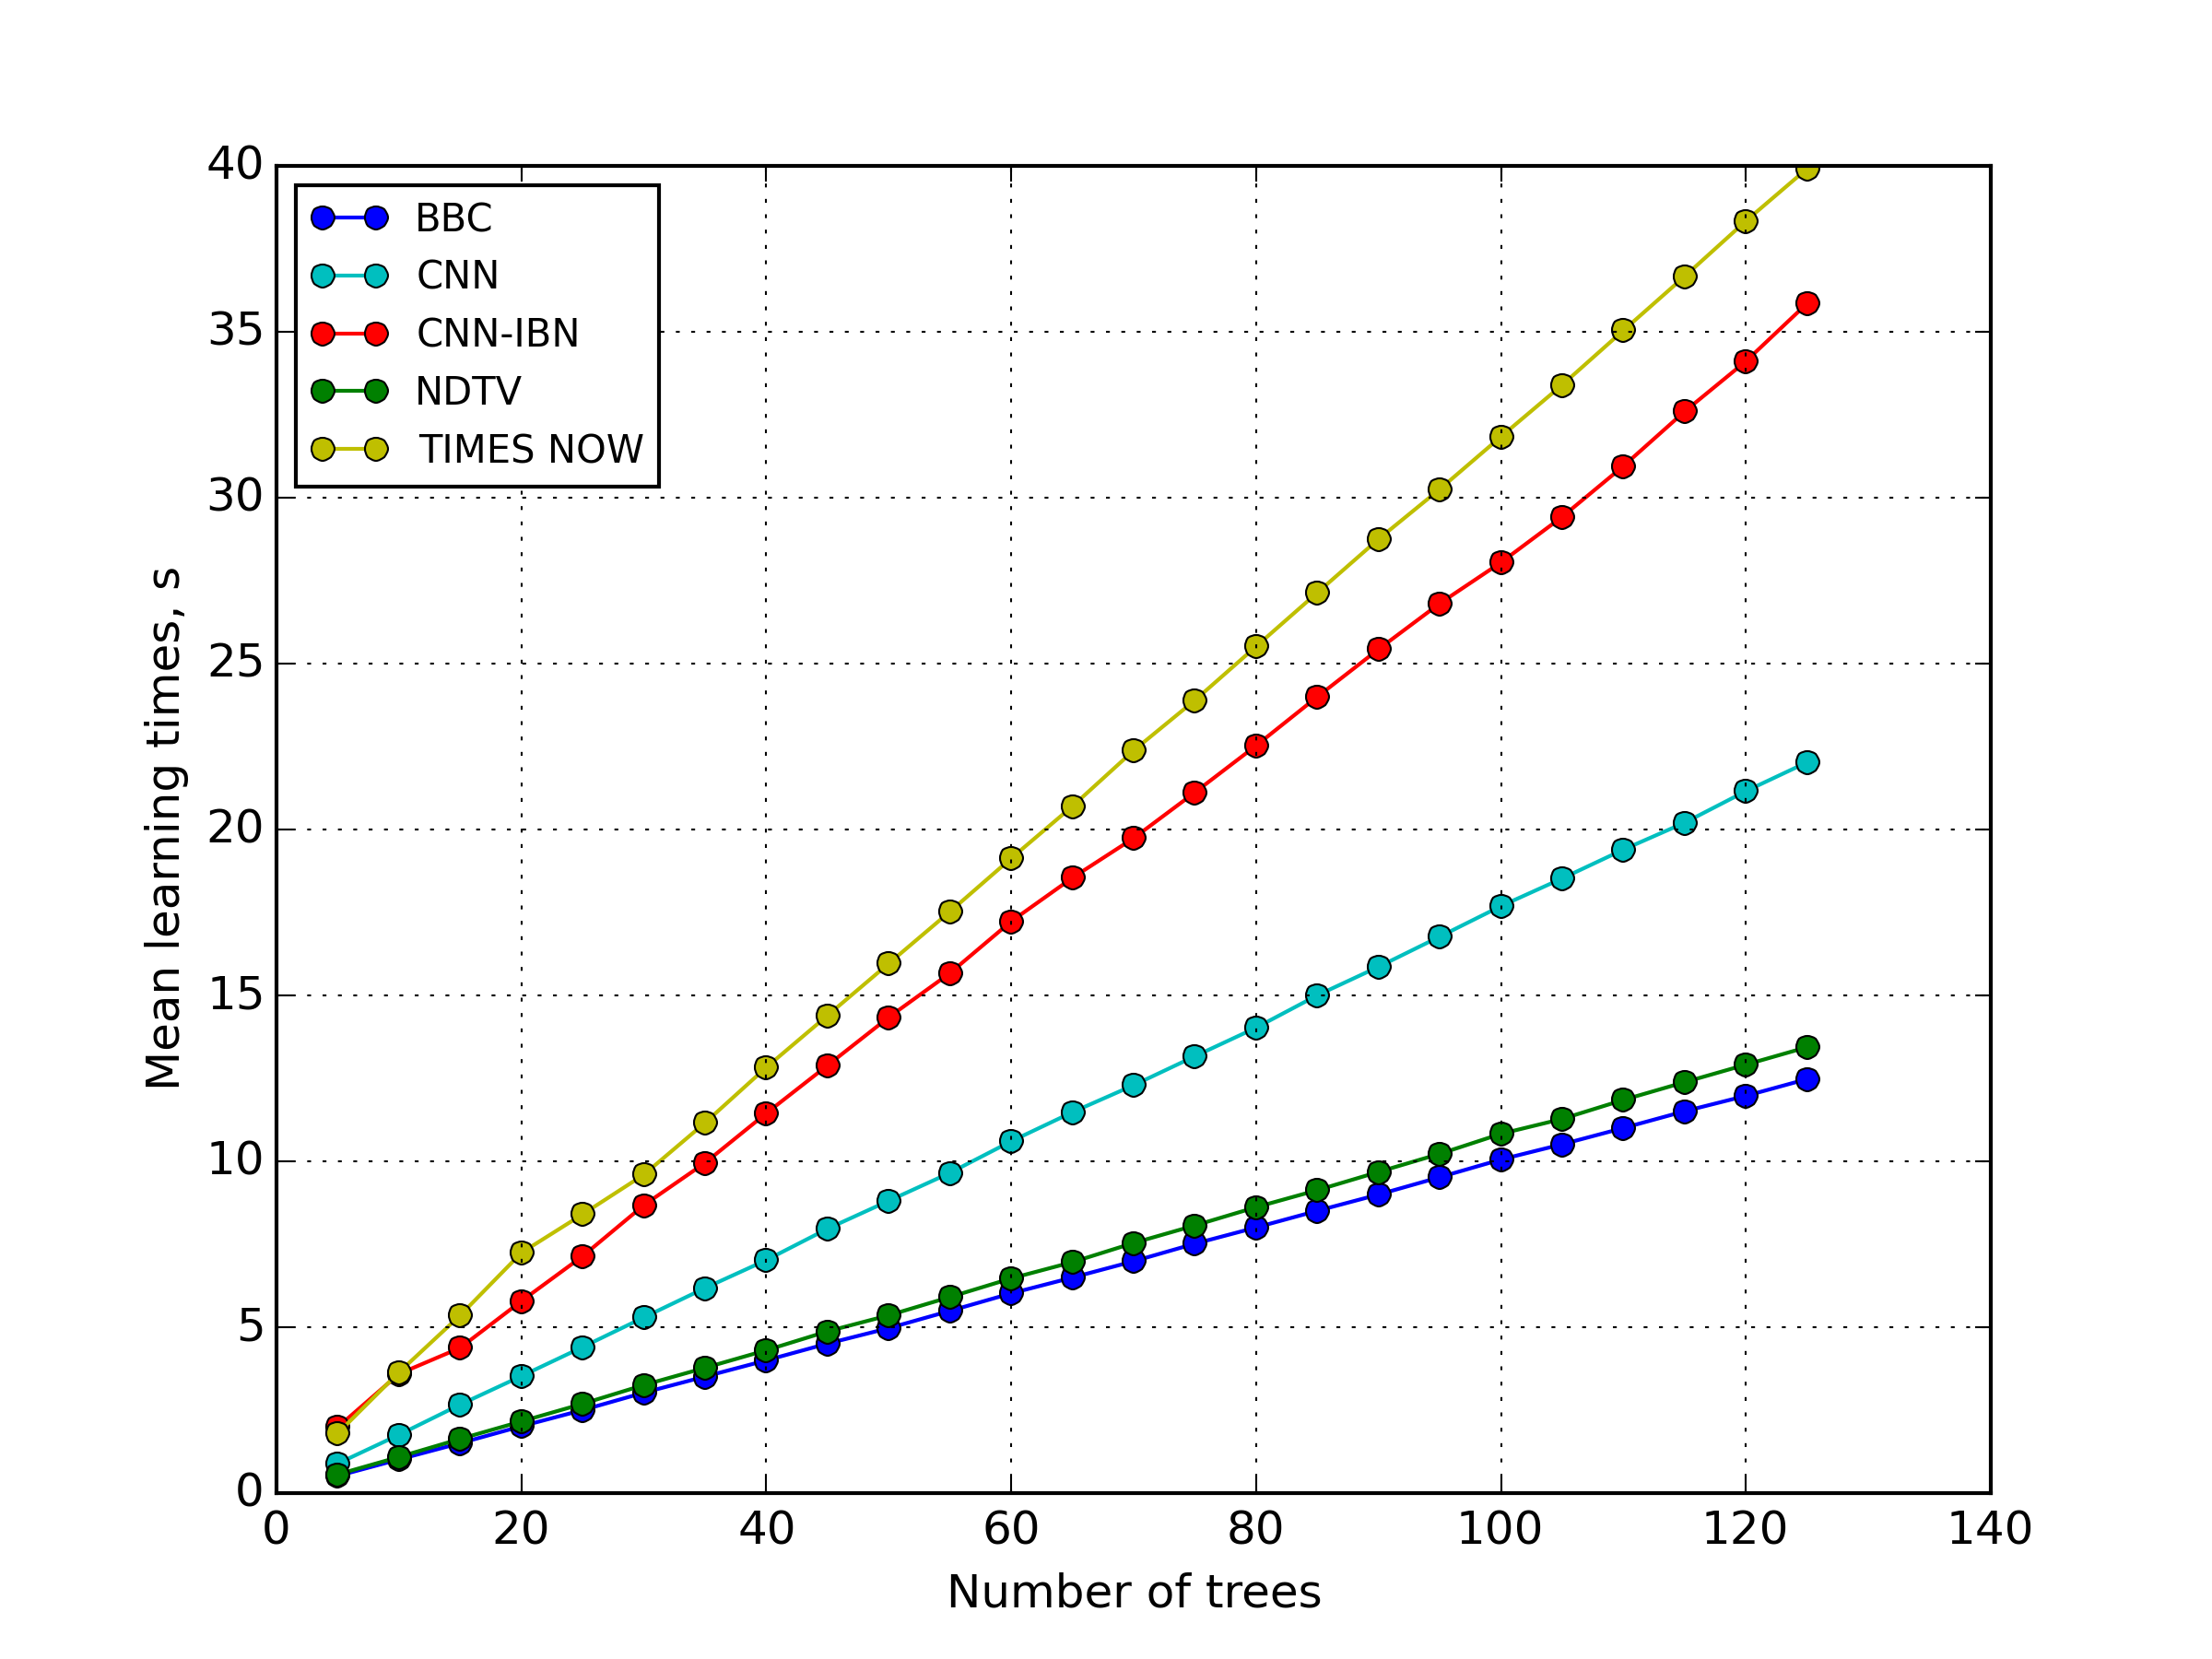
\includegraphics[width=\textwidth]{images/randforTime.png}
		\caption{Зависимости времён обучения для разных каналов.}
	\end{subfigure}
	\caption{Результаты для случайного леса}\label{fig:randfor-base}
\end{figure}

\tbd{Что мы видим на графиках?}

\subsubsection{Градиентный бустинг деревьев решений}
Бустинг --- мета-алгоритм, который итеративно добавляет в модель <<слабые>> подмодели (модель, предсказаниея которай слабо коррелирует с истинной классификацией, но показывает лучший результат, чем случайный выбор класса). Градиентный бустинг добавляет подмодели таким образом так, чтобы минимизировать некоторую дифференцируемую функцию потерь. Пусть к началу \(m\)-ой итерации ГБ построил модель, обладающую решающим правилом \(F_{m-1}(\mathbf{x})\). Если он выберет \(m\)-ую модель идеально, то \(F_{m}(\mathbf{x})=F_{m-1}(\mathbf{x}) + h_m(\mathbf{x})=y\), или иначе \(h_m(\mathbf{x})=y-F_{m-1}(\mathbf{x})\). Таким образом, ГБ на каждой итерации обучает новую подмодель на выборке \(\left(X, \{y_i-F_{m-1}(\mathbf{x}_i):y_i\in Y\}\right)\). Для квадратичной функции потерь \(L\left(y, F\right)=\frac12 \left(y-F(\mathbf{x})\right)^2\) остатки \(y-F_{m-1}(\mathbf{x})\) есть антиградиенты функции потерь, и метод, по сути, является градиентным спуском. Аналогично, для произвольной дифференцируемой функции потерь обучение \(m\)-ой подмодели на выборке с остатками вместо меток классов является реализацией градиентного спуска относительно функции потерь. Кроме этого, ГБ вычисляет коэффициент для решающего правила \(h_m(\mathbf{x})\), минимизируя функцию потерь вдоль направления антиградиента, и таким образом реализует наискорейший градиентный спуск.

Градиентый бустинг деревьев решений является реализацией ГБ для подмоделей в виде деревьев решений. Возможна модификация метода, которая позволяет улучшить качество классификации отдельных деревьев: вместо одного коэффициента для каждого решающего правила \(h_m(\mathbf{x})\) подбирать коэффициенты для каждого листа дерева. Такой алгоритм называется TreeBoost.

Для предотвращения переобучения подмоделей в градиентном бустинге могут применяться техники регуляризации: подбор числа итераций, модификация обновления решающего правила модели с помощью введения коэффициента \(\nu\) перед \(h_m(\mathbf{x})\), меньшего 1, в некотором смысле замедляющего построение модели (shrinkage).

Результаты запусков с различным числом деревьев представлены на рис.~\ref{fig:gtb-base}. Число деревьев \(M\) выбиралось из множества \(\{50,60,\dotsc,150\}\).
\begin{figure}[h!]
    \centering
	\begin{subfigure}{0.45\textwidth}
		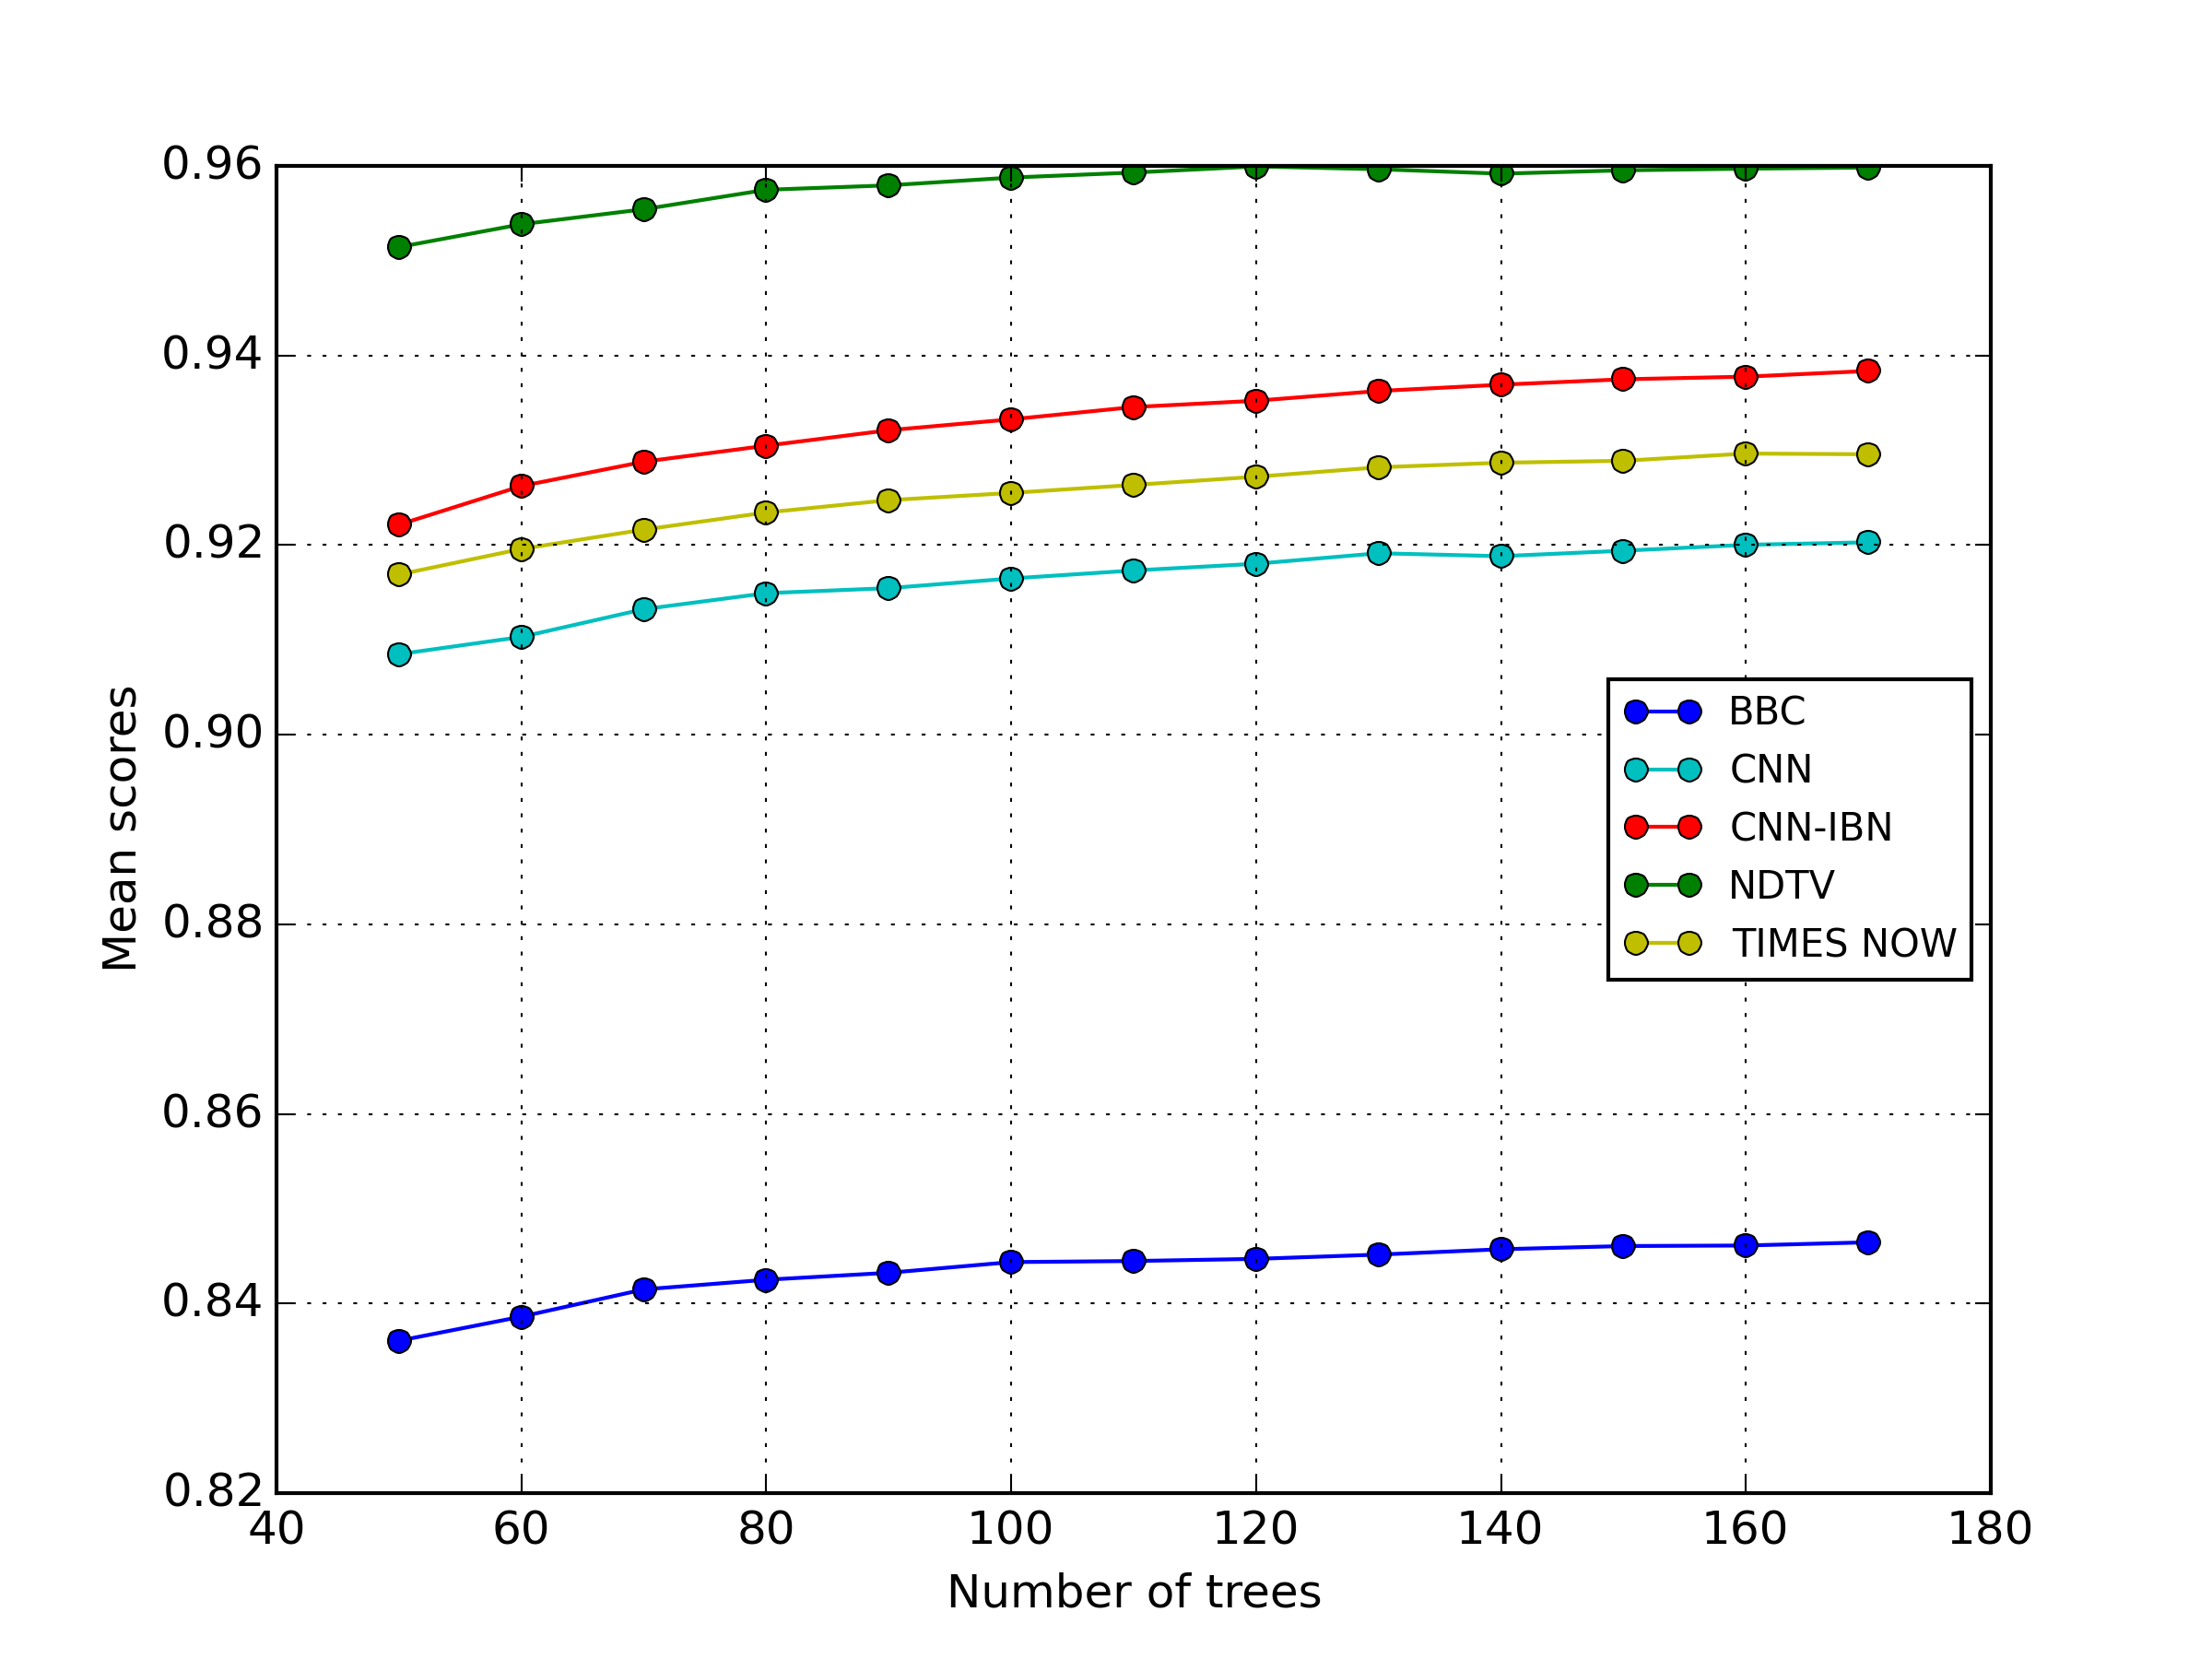
\includegraphics[width=\textwidth]{images/gtb.png}
		\caption{Зависимости качества классификации от числа деревьев для разных каналов.}
	\end{subfigure}
	\begin{subfigure}{0.45\textwidth}
		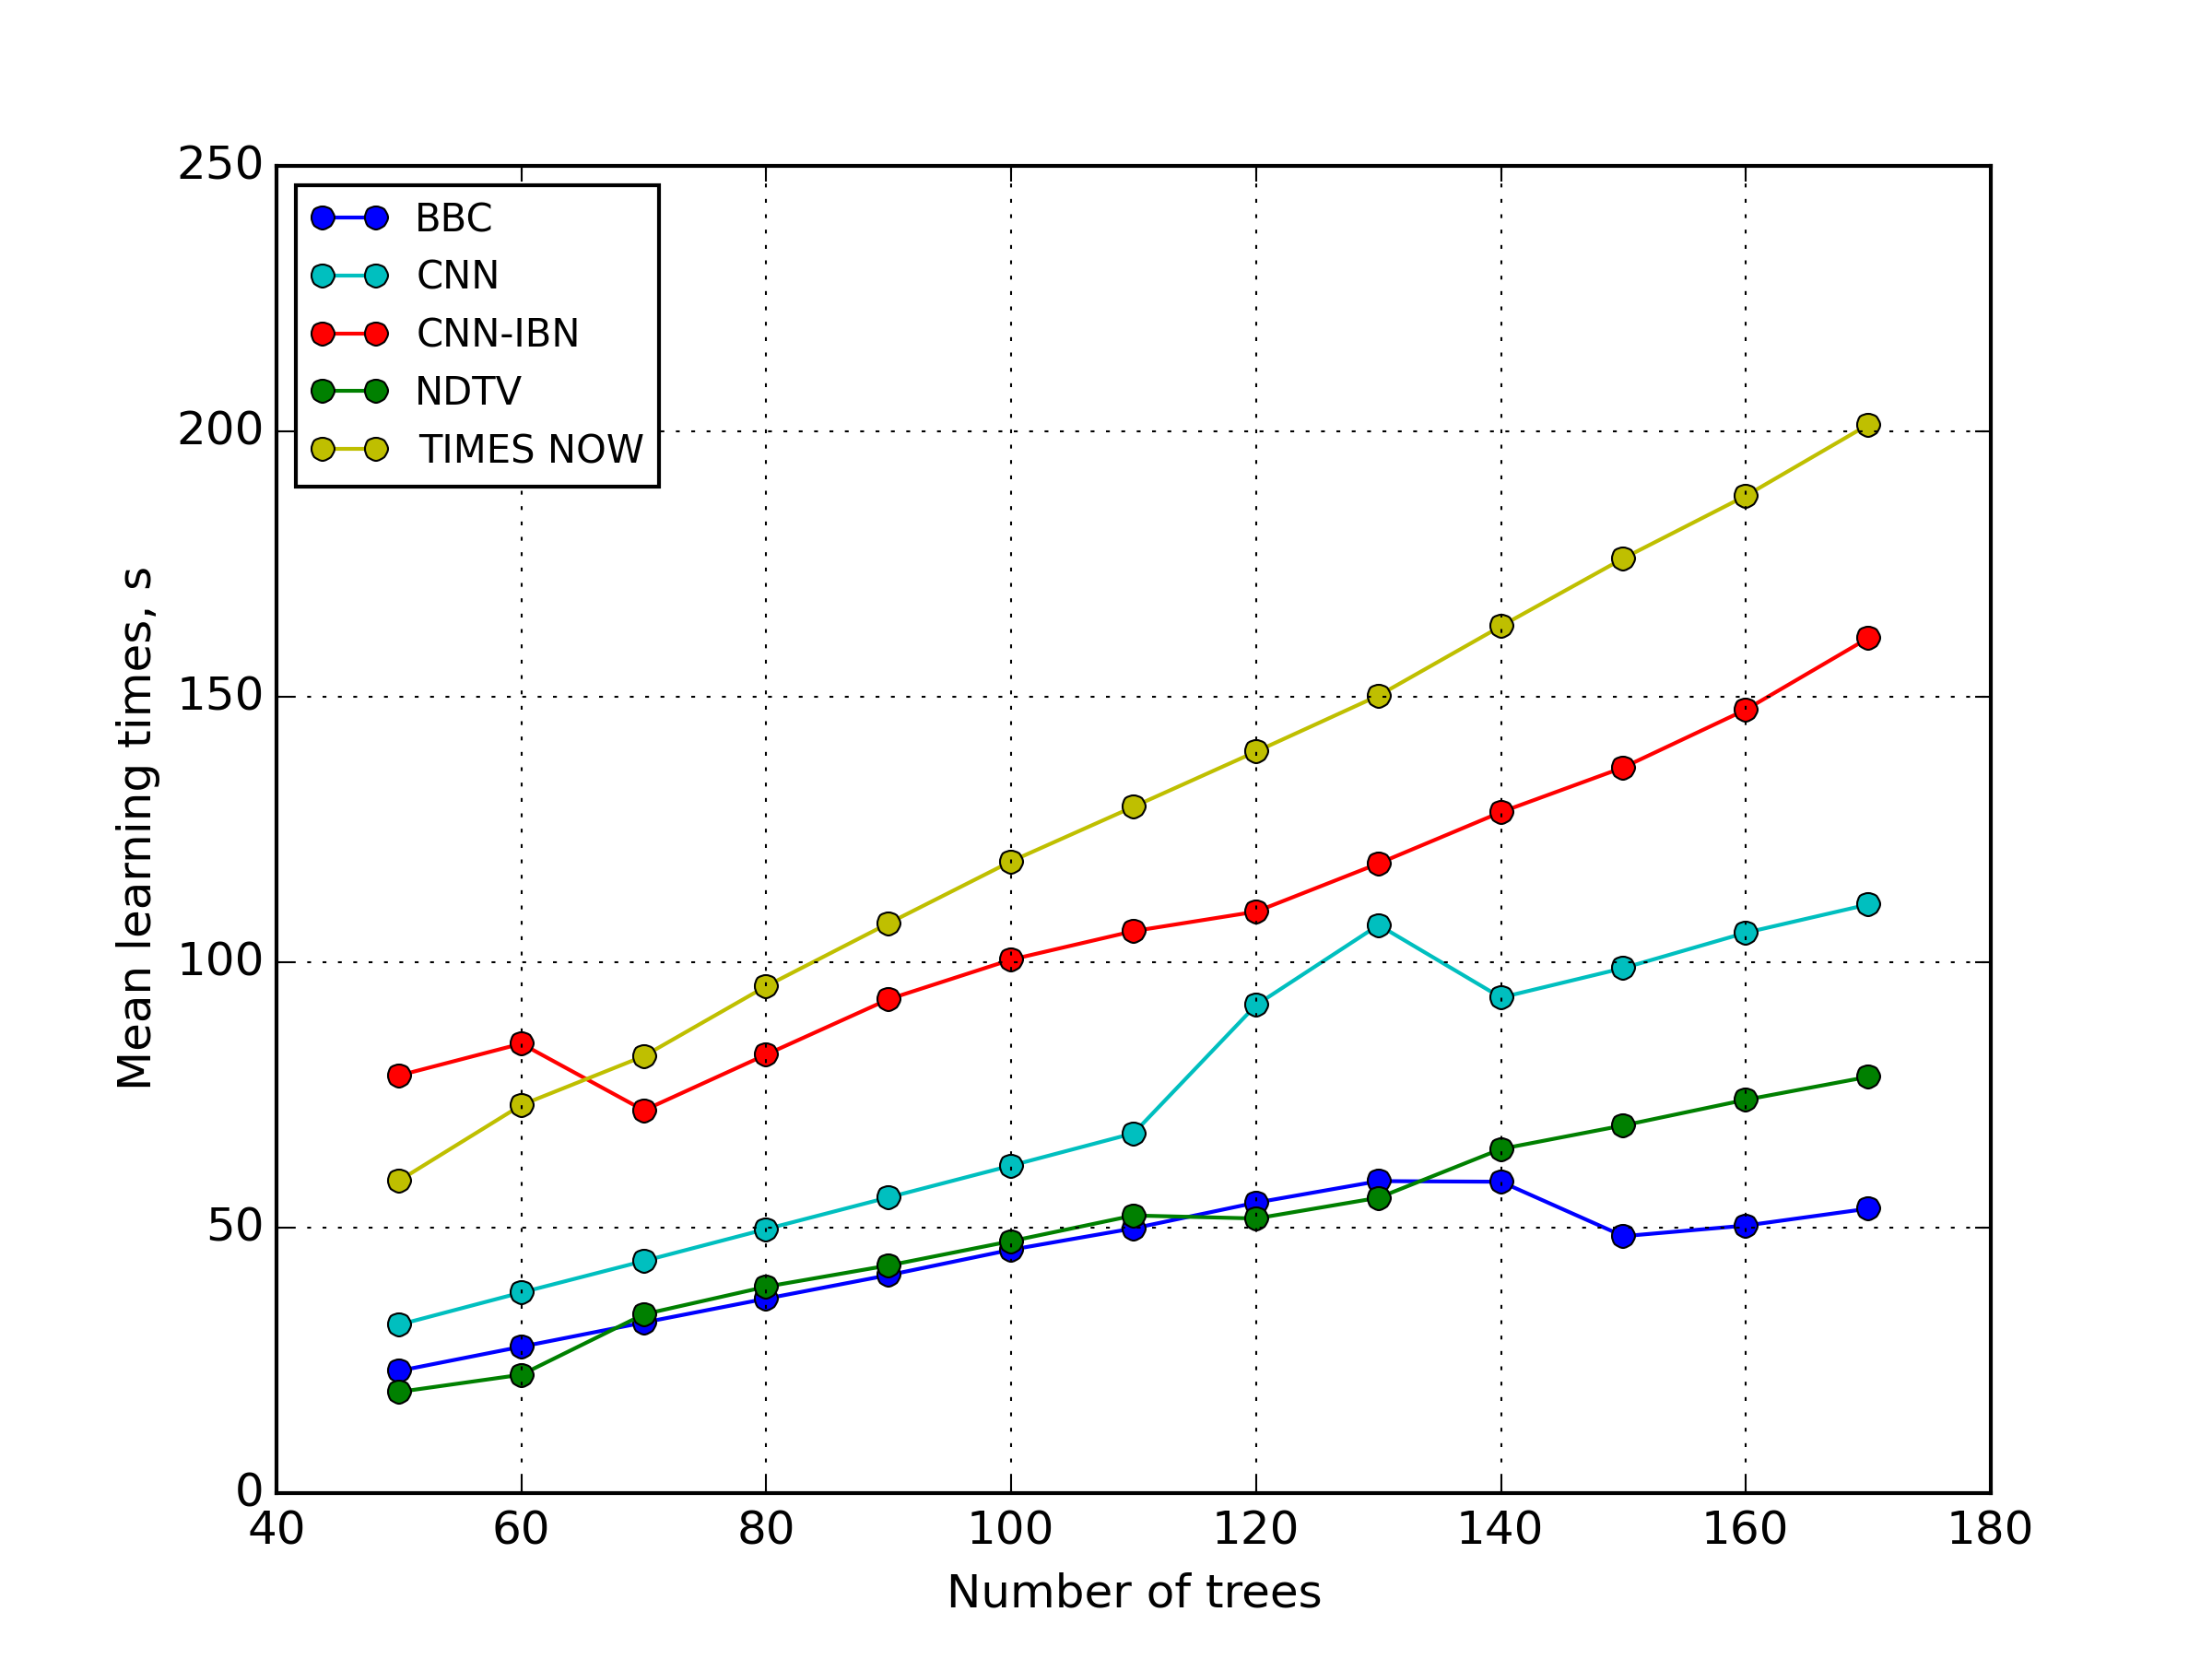
\includegraphics[width=\textwidth]{images/gtbTime.png}
		\caption{Зависимости времён обучения для разных каналов.}
	\end{subfigure}
	\caption{Результаты для градиентного бустинга деревьев решений}\label{fig:gtb-base}
\end{figure}

\tbd{Что мы видим на графиках?}

\subsubsection{Результаты для выбранных параметров}
В результате использования методов, описанных в данном разделе, были выбраны параметры, с которыми они будут запускаться после отбора признаков или эталонов. А именно, далее будут использоваться метод 15 ближайших соседей, случайный лес с 60 деревьями, SVM с \(C=4\) и градиентный бустинг со 100 деревьями. В таблице~\ref{table:base-all} сведена вся информация о качестве классификации и производительности методов для выбранных значений параметров.

\begin{table}[h!]
    \centering
    \begin{tabular}{|c||c|c|c|c|c|}
    \cline{2-6}
    \multicolumn{1}{c||}{} & \(k\)NN & LDA & Random forest & SVM & GTB \\
    \hline \hline
    CNN & \tworowcell{\(Q=78\%\)}{\(T_{train}=0.32 s\)} & \tworowcell{\(Q=90.4\%\)}{\(T_{train}=0.006 s\)} & \tworowcell{\(Q=92.2\%\)}{\(T_{train}=15.8 s\)} & \tbd{No data yet} & \tbd{No data yet} \\ \hline
    BBC & \tworowcell{\(Q=77.2\%\)}{\(T_{train}=0.37 s\)} & \tworowcell{\(Q=84.2\%\)}{\(T_{train}=0.003 s\)} & \tworowcell{\(Q=85.4\%\)}{\(T_{train}=9.3 s\)} & \tbd{No data yet} & \tbd{No data yet} \\ \hline
    CNN-IBN & \tworowcell{\(Q=79.6\%\)}{\(T_{train}=0.6s\)} & \tworowcell{\(Q=91.8\%\)}{\(T_{train}=0.1s\)} & \tworowcell{\(Q=94.4\%\)}{\(T_{train}=22.4s\)} & \tbd{No data yet} & \tbd{No data yet} \\ \hline
    TIMES NOW & \tworowcell{\(Q=76.1\%\)}{\(T_{train}=0.67s\)} & \tworowcell{\(Q=91.7\%\)}{\(T_{train}=0.1s\)} & \tworowcell{\(Q=93\%\)}{\(T_{train}=28.6s\)} & \tbd{No data yet} & \tbd{No data yet} \\ \hline
    NDTV & \tworowcell{\(Q=83.8\%\)}{\(T_{train}=1.15s\)} & \tworowcell{\(Q=93.3\%\)}{\(T_{train}=0.17s\)} & \tworowcell{\(Q=95.4\%\)}{\(T_{train}=9.5s\)} & \tbd{No data yet} & \tbd{No data yet} \\ \hline
    \end{tabular}
    \caption{Сводная таблица результатов базовых методов}
    \label{table:base-all}
\end{table}

